\documentclass[journal,12pt,twocolumn]{IEEEtran}

\makeatletter
\makeatother
\usepackage{setspace}
\usepackage{gensymb}
\usepackage{xcolor}
\usepackage{caption}

\singlespacing



\usepackage{graphicx}
\graphicspath{ {./images}  }

\usepackage[cmex10]{amsmath}
\usepackage{mathtools}
\usepackage{wasysym}
\usepackage{amsthm}
\usepackage{mathrsfs}
\usepackage{txfonts}
\usepackage{stfloats}
\usepackage{cite}
\usepackage{cases}
\usepackage{mathtools}
\usepackage{subfig}
\usepackage{enumerate}	
\usepackage{enumitem}
\usepackage{amsmath}

\usepackage{longtable}
\usepackage{multirow}

\usepackage{enumitem}
\usepackage{mathtools}
\usepackage{listings}
\usepackage{listings}
\usepackage[latin1]{inputenc}                               
\usepackage{color}                                           
\usepackage{array}                                         
\usepackage{longtable}                                    
\usepackage{calc}                                          
\usepackage{multirow}                                        
\usepackage{hhline}                                          
\usepackage{ifthen}                                           
\usepackage{lscape}     

\DeclareMathOperator*{\Res}{Res}

\renewcommand\thesection{\arabic{section}}
\renewcommand\thesubsection{\thesection.\arabic{subsection}}
\renewcommand\thesubsubsection{\thesubsection.\arabic{subsubsection}}
\hyphenation{op-tical net-works semi-conduc-tor}

\def\inputGnumericTable{}                               

\lstset{
frame=single, 
breaklines=true,
columns=fullflexible
}

 

\begin{document}

\theoremstyle{definition}
\newtheorem{theorem}{Theorem}[section]
\newtheorem{problem}{Problem}
\newtheorem{proposition}{Proposition}[section]
\newtheorem{lemma}{Lemma}[section]
\newtheorem{corollary}[theorem]{Corollary}
\newtheorem{example}{Example}[section]
\newtheorem{definition}{Definition}[section]

\newcommand{\BEQA}{\begin{eqnarray}}
\newcommand{\EEQA}{\end{eqnarray}}
\newcommand{\define}{\stackrel{\triangle}{=}}

\bibliographystyle{IEEEtran}

\providecommand{\nCr}[2]{\,^{#1}C_{#2}} % nCr
\providecommand{\nPr}[2]{\,^{#1}P_{#2}} % nPr
\providecommand{\mbf}{\mathbf}
\providecommand{\pr}[1]{\ensuremath{\Pr\left(#1\right)}}
\providecommand{\qfunc}[1]{\ensuremath{Q\left(#1\right)}}
\providecommand{\sbrak}[1]{\ensuremath{{}\left[#1\right]}}
\providecommand{\lsbrak}[1]{\ensuremath{{}\left[#1\right.}}
\providecommand{\rsbrak}[1]{\ensuremath{{}\left.#1\right]}}
\providecommand{\brak}[1]{\ensuremath{\left(#1\right)}}
\providecommand{\lbrak}[1]{\ensuremath{\left(#1\right.}}
\providecommand{\rbrak}[1]{\ensuremath{\left.#1\right)}}
\providecommand{\cbrak}[1]{\ensuremath{\left\{#1\right\}}}
\providecommand{\lcbrak}[1]{\ensuremath{\left\{#1\right.}}
\providecommand{\rcbrak}[1]{\ensuremath{\left.#1\right\}}}
\theoremstyle{remark}
\newtheorem{rem}{Remark}
\newcommand{\sgn}{\mathop{\mathrm{sgn}}}
\providecommand{\abs}[1]{\left\vert#1\right\vert}
\providecommand{\res}[1]{\Res\displaylimits_{#1}} 
\providecommand{\norm}[1]{\lVert#1\rVert}
\providecommand{\mtx}[1]{\mathbf{#1}}
\providecommand{\mean}[1]{E\left[ #1 \right]}
\providecommand{\fourier}{\overset{\mathcal{F}}{ \rightleftharpoons}}
\providecommand{\system}{\overset{\mathcal{H}}{ \longleftrightarrow}}

\newcommand{\solution}{\noindent \textbf{Solution: }}
\providecommand{\dec}[2]{\ensuremath{\overset{#1}{\underset{#2}{\gtrless}}}}
\DeclarePairedDelimiter{\ceil}{\lceil}{\rceil}
\numberwithin{equation}{section}

\let\StandardTheFigure\thefigure

\let\StandardTheFigure\thefigure
\let\StandardTheTable\thetable

\def\putbox#1#2#3{\makebox[0in][l]{\makebox[#1][l]{}\raisebox{\baselineskip}[0in][0in]{\raisebox{#2}[0in][0in]{#3}}}}
     \def\rightbox#1{\makebox[0in][r]{#1}}
     \def\centbox#1{\makebox[0in]{#1}}
     \def\topbox#1{\raisebox{-\baselineskip}[0in][0in]{#1}}
     \def\midbox#1{\raisebox{-0.5\baselineskip}[0in][0in]{#1}}

\title{ Support Vector Machine}

\author{Nisha Akole, G V V 
Sharma$^{*}$% <-this % stops a space
\thanks{*The authors are with the Department
of Electrical Engineering, Indian Institute of Technology, Hyderabad
502285 India e-mail:  gadepall@iith.ac.in.}
}

\maketitle

\tableofcontents

\bigskip
\begin{abstract}
This manual provides a brief description on how to implement Support Vector Machine, a classifier technique.
\end{abstract}

\IEEEpeerreviewmaketitle

\section{Objective}

Our objective is perform classification of datasets and decide class for new data points. 
\section{Load Dataset}
Download the dataset file from following link in the folder where you want to write code for SVM.
\begin{lstlisting}
https://github.com/prabhatrai111/Commensal-Radar
\end{lstlisting}

\section{About SVM}
Support Vector Machine(SVM) is supervised machine learning algorithm which can be used for both classification or regression challenges. It is well known for its kernels, to classify non-linear data. SVM known as a discriminative classifier as it separates data points using a hyperplane with large margin.\\
\begin{itemize}
\item Support Vector:\\
	These are the data points closest to hyperplane and helps to define a proper margin.\\
\item Hyperplane:\\
	A plane which separates set of objects into different classes.\\
\item Margin:\\
	A distance from hyperplane which separates classes. Larger margin is considered as good for classification and avoids overlapping.
\end{itemize}

SVM can be divided into two types based on dataset and kernel used to classify it


\subsection{Simple SVM}
In Simple SVM, parameters are linear. Kernel used is also a linear kernel to classify a linear data.

\begin{lstlisting}
link for linear kernel code
\end{lstlisting}

\subsection{Kernel SVM}
Kernel SVM is used specially to classify non-linear data by using different kernels such as polynomial, gaussian radial basis function(rbf) and sigmoid.
 
\begin{lstlisting}[mathescape=true]
link for 2 non-linear kernel code
\end{lstlisting}

\section{Evaluating the Algorithm}
Confusion matrix, accuracy, precision and recall are metrices used for checking the algorithm correctness. Scikit-learn is a free machine learning library for python, mostly used for various algorithms like support vector machine, principal component analysis, random forest etc. Sklearn contains classification\_report and confusion\_matrix for classification tasks.

\section{Tuning Hyperparameters}
\begin{itemize}
\item Kernel: SVM will give different output for different kernels. Use of kernel is totally dependent on the type of dataset. To get optimized output, one has to test different kernels for the good results.\\
	
\item Regularization Parameter(C): It is used to calculate error and helps to reduce it. C is also used to decide margin. A small value of C will create a small margin around hyperplane and large value will create large margin. By this parameter, we cancontrols trade off between smooth decision boundary and error.\\


\item Gamma: A lower value of gamma will underfit the data and higher value of gamma will overfit the data.\\

\end{itemize}


\section{SVM Pros and Cons}
\subsection{Pros}
\begin{itemize}
\item Works really well when no. of dimensions is greater than no. of samples i.e effective in high dimensional spaces.
\item It gives good accuracy and uses less memory because they use a subset training points in the decision phase.
\item SVM works well with clear margin of separation.
\item Risk of overfitting is less in SVM.
\end{itemize}


\subsection{Cons}
\begin{itemize}
\item It takes more time for training. Hence, not suitable for large datasets.
\item Works poorly with overlapping classes and also type of kernel used will also affect the output of SVM. Choosing good kernel is not easy.
\item The SVM hyper-parameters are cost and gamma. It is hard to visualize their effect.
\end{itemize}

\section{Figures}
\begin{figure}[!h]
\begin{center}
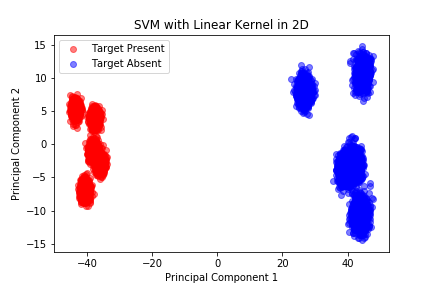
\includegraphics[width=3.5in]{figs/LinSVM_2D.png}
\end{center}
\caption{SVM with Linear Kernel in 2D}
\label{fig: 2D Plot}
\end{figure}

\begin{figure}[!h]
\begin{center}
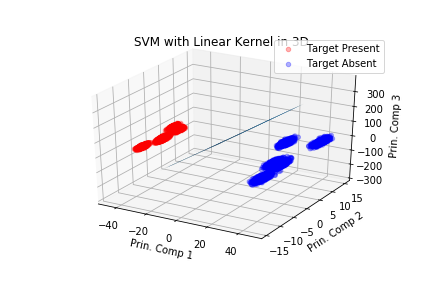
\includegraphics[width=3.9in]{figs/LinSVM_3D.png}
\end{center}
\caption{SVM with Linear Kernel in 3D}
\label{fig: 3D Plot}
\end{figure}

\begin{figure}[!h]
\begin{center}
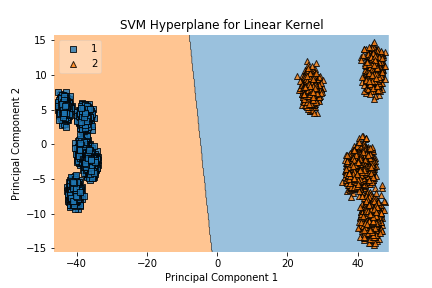
\includegraphics[width=3.8in]{figs/HyperPlane_Lin.png}
\end{center}
\caption{SVM Hyperplane for Linear Kernel}
\label{fig: 3D Plot}
\end{figure}

\begin{figure}[!h]
\begin{center}
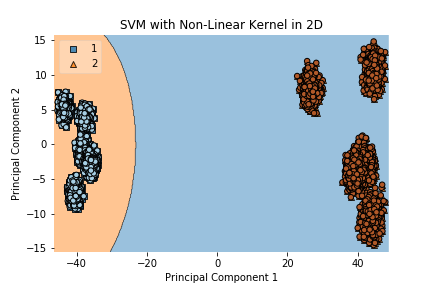
\includegraphics[width=3.8in]{figs/NLinSVM_2D.png}
\end{center}
\caption{SVM for Non-linear Kernel}
\label{fig: 3D Plot}
\end{figure}

\begin{figure}[!h]
\begin{center}
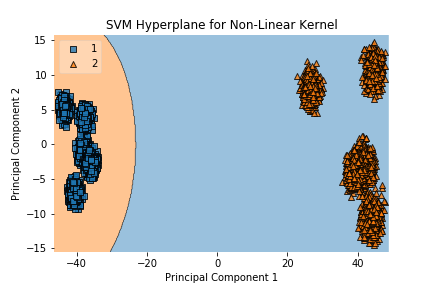
\includegraphics[width=3.8in]{figs/HyperPlane_NLin.png}
\end{center}
\caption{SVM Hyperplane for Non-linear Kernel}
\label{fig: 3D Plot}
\end{figure}



\end{document}

© 2019 GitHub, Inc.
Terms
Privacy
Security
Status
Help
Contact GitHub
Pricing
API
Training
Blog
About